\section{Resoconto attività di verifica} \label{_resocontoVerifica}
\subsection{Revisione dei requisiti}
\subsubsection{Analisi statica dei documenti}
Tutta la documentazione prodotta in ingresso alla Revisione dei Requisiti è stata sottoposta ad una meticolosa attività di verifica
basata su quanto previsto all'interno del documento delle norme di progetto.
Questa attività è stata espletata dai verificatori.

\subsubsection{Analisi automatizzata dei documenti}
Al fine di verificare la qualità della documentazione prodotta il gruppo ha deciso di adottare come metrica di verifica
l'indice di Gulpease generato grazie ad un processo automatizzato configurato in \textit{\glock{GitHub}}, unitamente alla generazione di un indice di 
correttezza grammaticale del testo.
Di seguito sono presentati i due grafici rappresentativi dei valori ottenuti dall'analisi dei documenti sino all'approvazione degli stessi.
Per quanto riguarda i verbali redatti in occasione dei meeting tra i membri del gruppo e con i proponenti si espongono i valori in forma tabellare


\begin{center}
   
		\begin{figure}[!htb]
			\centering
			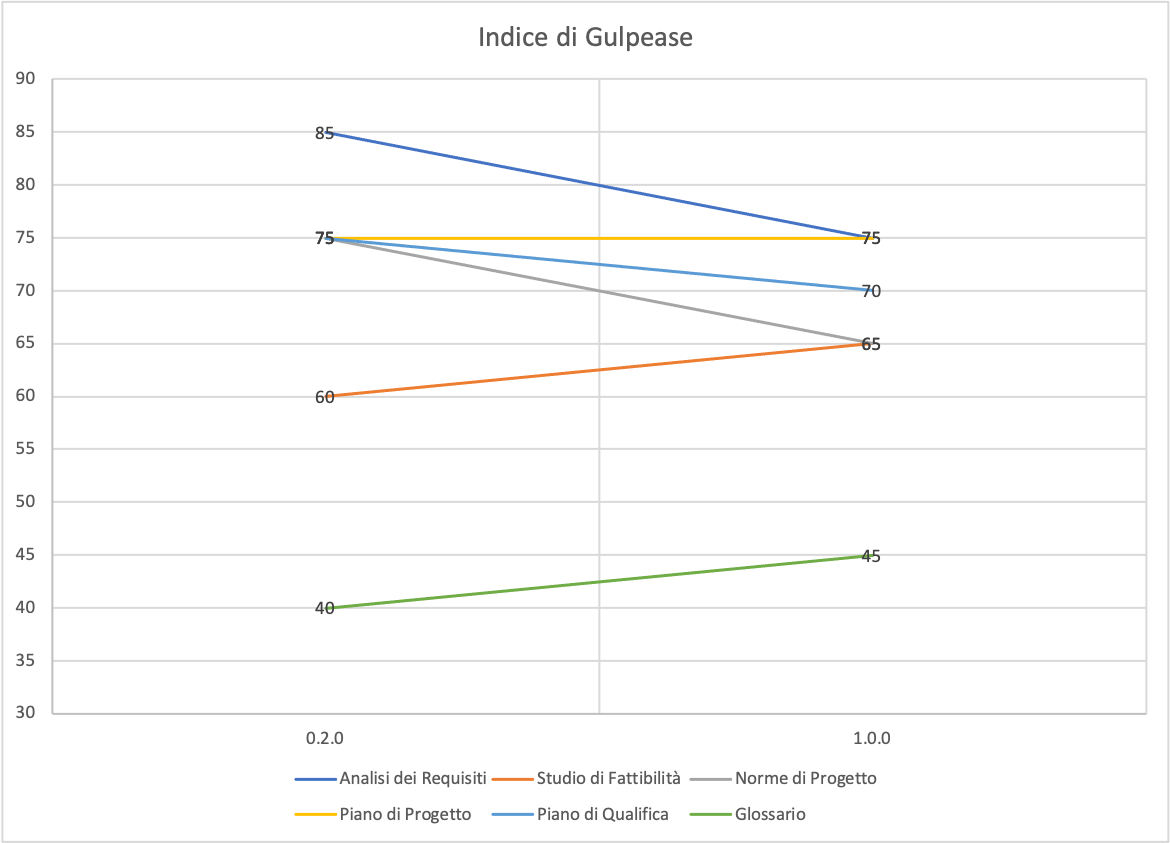
\includegraphics[scale=0.80]{res/images/grafico_gulpease.png}	
			\caption{Grafico Indice di Gulpease}
        \end{figure}
        

        \begin{figure}[!htb]
			\centering
			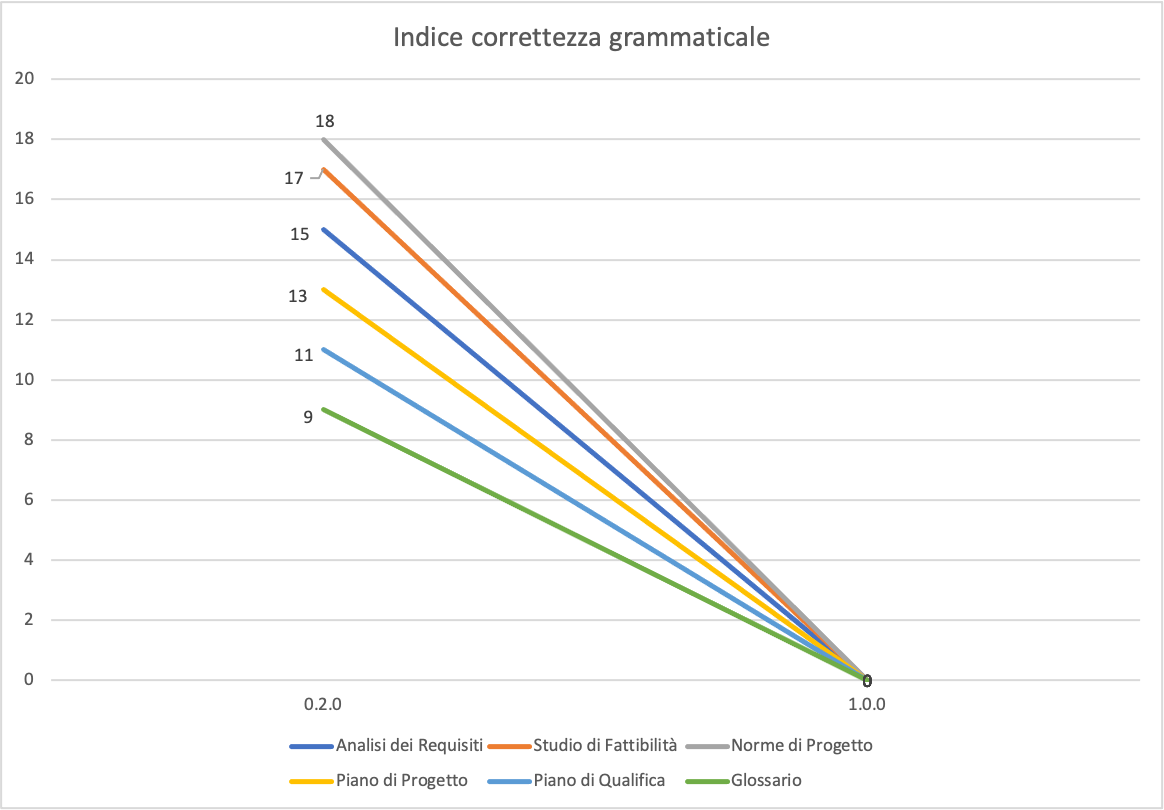
\includegraphics[scale=0.80]{res/images/grafico_correttezza.png}	
			\caption{Grafico indice correttezza grammaticale}
		\end{figure}
	




    \begin{center}
        \rowcolors{2}{white}{blue!20}
        
        \begin{longtable}{|c|c|}
      
        \hline
        \rowcolor{lighter-grayer}
        \textbf{Documento} & \textbf{Indice di Gulpease} \\
       
        \hline
        \endfirsthead


        \hline


       
      

        Verbale Interno 2020-11-24 & 77 \\
        Verbale Interno 2020-12-05 & 70 \\
        Verbale Interno 2020-12-07& 71 \\
        Verbale Esterno 2020-12-10 & 73  \\
        Verbale Interno 2020-12-14 & 72 \\
        Verbale Interno 2020-12-17 & 75  \\
        Verbale Interno 2020-12-22 & 70 \\
        Verbale Interno 2020-12-28 & 73  \\
        Verbale Interno 2021-01-02& 73 \\  
        Verbale Esterno 2021-01-08 & 74  \\
        

    
        \hline
        \rowcolor{white}
        \caption{Indice di Gulpease dei verbali}
        
        \end{longtable}
    \end{center}
\end{center}


